\documentclass[letterpaper,titlepage]{article}
\usepackage{Amish_Style}

\title{Matrix Chain Multiplication Project Report}
\author{Amish Mishra}
\date{Due: April 24, 2021}

\begin{document}
\maketitle

\section{Problem Definition}\label{def}
Given a sequence (chain) of matrices with compatible dimensions $\langle A_1,A_2, \dots, A_n\rangle$ to be multiplied, in what order should we parenthesize the matrices to minimize the total number of scalar multiplications needed to yield the result? Since matrix multiplication is associative, we can place parentheses anywhere. However, some ways of parenthesizing the sequence of matrices yield the product faster than other ways.
\newline
\newline
\textbf{Input:} $p$, an array of length $n+1$ where $n$ is the number of matrices. $p$ has the dimensions of the matrices to be multiplied. So, $p[0]$ and $p[1]$ are the number of rows and columns of matrix $A_1$ respectively. Then, $p[1]$ and $p[2]$ are the number of rows and columns of matrix $A_2$, respectively. And so on and so forth.
\newline
\textbf{Output:} $m$ and $s$ where $m$ is the minimum number of scalar multiplications done for an optimal solution and $s$ contains the parenthesization of the matrices $\langle A_1,A_2, \dots, A_n\rangle$.

\section{Application}
A matrix can also be viewed as a linear transformation from one vector space, say $\R^n$ to another vector space $\R^k$. In finite dimensions, a linear transformation can be written as a matrix \cite{Chen}. Thus, when considering a sequence of linear transformations
    $$T_1T_2\dots T_n.$$
We may write them as a product of their associated matrices
    $$A_1A_2\dots A_n.$$
Computing such a product is a matrix chain multiplication problem.


\section{Algorithms}
In this project, I implemented and analyzed two algorithms:
\begin{enumerate}
    \item Brute-Chain (Brute-Force)
        \subitem This algorithm exhaustively checks all possible parenthesizations. It then returns the minimum number of multiplications done over all possible parenthesizations. This algorithm has a worst-case run-time of $\Omega(2^n)$ \cite{CLRS}. The pseudo-code in this report is adapted from R. Muhammad \cite{muhammad}.
    \item Dynamic-Chain (Dynamic Programming)
        \subitem This algorithm makes use of the type of problem we have, which has the optimal solution determined by finding optimal solutions of subproblems and many subproblems overlap. Thus, we use dynamic programming which stores the results of expensive computations for use again when the same computation needs to be run. In our case, as we look to find an optimal parenthesization, we will end up multiplying the same dimension matrices over and over. Thus, using a look-up table saves much computation time and brings the run-time down to $\Omega(n^3)$. This pseudo-code in this report is adapted from the CLRS book \cite{CLRS}.
\end{enumerate}

\subsection{Pseudo-code}
\begin{lstlisting}[language=Python]
# declare m and s global for Brute-Chain to access on any level of recursion
global m, s  
Brute-Chain(p, i, j):
    if i == j:
        m[i, j] = 0
    else:
        m[i, j] = np.infty
        for k in range(i, j):
            c = brute_chain(p, i, k) + brute_chain(p, k+1, j) + p[i]*p[k+1]*p[j+1]
            if c < m[i, j]:
                m[i, j] = c
                s[i, j] = k
    return m[i, j]

Call-Brute-Chain():
    m, s = Brute-Chain(p, 0, length(p)-2) # function call
    return m and s
        

Dynamic-Chain(p)
    n = p.length-1
    let m[1..n,1..n] and s[1..n-1,2..n] be new tables
    for i = 1 to n
        m[i,i] = 0
    for l = 2 to n  // l is the chain length
        for i = 1 to n-l+1
            j = i + l - 1
            m[i,j] = infinity
            for k = i to j - 1
                q = m[i,k] + m[k+1,j] + p_{i-1}p_kp_j
                if q < m[i,j]
                    m[i,j] = q
                    s[i,j] = k
    return m and s
    
Print-Optimal-Parens(s,i,j)  // Printing function
    if i == j
        print "A"_i
    else print "("
       Print-Optimal-Parens(s,i,s[i,j])
       Print-Optimal-Parens(s,s[i,j]+1,j)
       print ")"
            

\end{lstlisting}
\subsection{Run-time Analysis}
The Brute-Chain algorithms runs in exponential time $\Omega(2^n)$. I first write the various ways to parenthesize a chain of length $n$ as a recurrence relation. I note that the ways to parenthesize a chain of length 1 is exactly 1, and the number of ways to parenthesize a chain of length more than 1 is the sum of the number of ways to parenthesize the sub-chains created by splitting the chain at position $k$. I have the formula for the number of ways to parenthesize a chain of length $n$ as $P(n)$:
\begin{equation*}
P(n) = \left\{
        \begin{array}{ll}
           1 & \quad n=1 \\
            \sum_{k=1}^{n-1} P(k)P(n-k) & \quad n \geq 2
        \end{array}
    \right.
\end{equation*}
I see that the base case holds since $1 \geq (1/4)2^n$ for $n=1.$ Now, I assume that there exists some constant $c$ such that $P(n) \geq c2^n$ for every $n \geq 2$. I perform the inductive step on $P(n+1)$:
$$P(n+1) = \sum_{k=1}^{n-1} P(k)P(n-k) \geq 2^n \sum_{k=1}^{n-1} 2c = 2(n-1)c2^n.$$
Thus, I have found a constant $2(n-1)c$ so that $2(n-1)c2^n$ is a lower bound for $P(n)$. Hence, I conclude that the run-time for Brute-Chain is $\Omega(2^n).$
\newline
The run-time analysis for Dynamic-Chain will be done directly from the pseudo-code. The first for-loop runs in $O(n)$ time. Then, the first level of the next for-loop runs in $O(n)$ time since $l$ ranges from 2 to $n$. The next level of the for-loop in the nest runs in $O(n)$ time. The next level of the for-loop nest runs in $O(n)$ time as well since $j$ can take on values close to $n$ while $i$ can take values close to $1$ simultaneously. Thus, the run-time of Dynamic-Chain is $O(n^3)$ due to the triple nested for-loop.

\section{Experiment Design}
I used the Python programming language and the Pycharm IDE for this project. The input size for my algorithms was $n$ - the number of matrices to be multiplied.
The data structure was a $1 \times n+1$ array of numbers representing the sequence of matrix dimensions being multiplied, as described in \ref{def}. For example, $[11,8,23,42]$ represents a $11\times 8$ matrix times an $8 \times 23$ matrix times a $23 \times 42$ matrix. The data structures involved in both Brute-Chain and Dynamic-Chain were 2 arrays, $m$ and $s$, to track the optimal values for each parenthesization and the parenthesization itself. When computing the run-time, I only computed the run-time of the raw algorithm as it built the two arrays, $m$ and $s$; I did not factor in the time to print out the final parenthesization of the chain or the optimal solution.

\subsection{Generating input}
Since the matrices themselves never get multiplied, I simply generate a sequence of positive numbers. I did this with a random function in python to generate a $1 \times n+1$ dimension array with entries between $3$ and $20$. I ensured I generated the input array and fed it to both algorithms before generating another one. I generated $5$ runs of $n+1$ length arrays for fixed $n$ and took the average run-time for the 5 runs. Then, I varied $n$ from $3$ to $16$ to have run-times for increasing sizes of chains.


\subsection{Brute-Chain}
The theoretical complexity for this algorithm is $\Omega(2^n)$, exponential. I expected there to be some constant in front of this to make the execution complexity $c_12^n$ due to Python's interpreter. I computed $c_1$ using dynamic analysis, that is by running the code. I used the values
$$n = 2,3,4,\dots,13,14.$$
I calculated the ratio of the actual run-time with the theoretical run-time ($2^n$) and took the max of the reasonable ratios to find $c_1$. I found the max ratio to be $c_1=0.00019458149327$ from the ``Ratio" column of Table ~\ref{table:brute-chain}.
\begin{table}
    \centering
    \begin{tabular}{|l|l|l|l|l|}
    \hline
        n & Theoretical Complexity ($2^n$) & Empirical-RT (sec) & Ratio & Predicted-RT \\ \hline
        2 & 4 & 9.29832458496094E-06 & 2.32458114624023E-06 & 0.000778325973079 \\ \hline
        3 & 8 & 2.07424163818359E-05 & 2.59280204772949E-06 & 0.001556651946157 \\ \hline
        4 & 16 & 5.76972961425781E-05 & 3.60608100891113E-06 & 0.003113303892314 \\ \hline
        5 & 32 & 0.000170278549194 & 5.321204662323E-06 & 0.006226607784629 \\ \hline
        6 & 64 & 0.000506782531738 & 7.91847705841064E-06 & 0.012453215569258 \\ \hline
        7 & 128 & 0.00151252746582 & 1.18166208267212E-05 & 0.024906431138516 \\ \hline
        8 & 256 & 0.004510688781738 & 1.76198780536652E-05 & 0.049812862277031 \\ \hline
        9 & 512 & 0.013286924362183 & 2.59510241448879E-05 & 0.099625724554062 \\ \hline
        10 & 1024 & 0.039701366424561 & 3.87708656489849E-05 & 0.199251449108124 \\ \hline
        11 & 2048 & 0.117401027679443 & 5.7324720546603E-05 & 0.398502898216248 \\ \hline
        12 & 4096 & 0.351414823532104 & 8.57946346513926E-05 & 0.797005796432495 \\ \hline
        13 & 8192 & 1.04952416419983 & 0.0001281157427 & 1.59401159286499 \\ \hline
        14 & 16384 & 3.18802318572998 & 0.00019458149327 & 3.18802318572998 \\ \hline
    \end{tabular}
    \caption{Tabular data for run-time analysis for Brute-Chain}
    \label{table:brute-chain}
\end{table}

\subsection{Dynamic-Chain}
The theoretical complexity for this algorithm is $\Omega(n^3)$. I expected there to be some constant in front of this to make the execution complexity $c_2n^3$ due to Python's interpreter. I computed $c_2$ using dynamic analysis, that is by running the code. I used the values
$$n = 9, 10, 11, 12, 13, 14.$$
I calculated the ratio of the actual run-time with the theoretical run-time ($n^3$) and took the max of the reasonable ratios to find $c_1$ (I omitted the first 7 rows because they appeared to be outliers). I found the max ratio to be $c_2=2.38353169340492*10^{-7}$ from the ``Ratio" column of Table ~\ref{table:dynamic-chain}.
\begin{table}
    \centering
    \begin{tabular}{|l|l|l|l|l|}
    \hline
        n & Theoretical Complexity ($n^3$) & Empirical-RT (sec) & Ratio & Predicted-RT \\ \hline
        2 & 8 & 7.91549682617188E-06 & 9.89437103271485E-07 & 7.91549682617188E-06 \\ \hline
        3 & 27 & 1.44481658935547E-05 & 5.35117255316841E-07 & 2.67148017883301E-05 \\ \hline
        4 & 64 & 2.54631042480469E-05 & 3.97861003875733E-07 & 6.3323974609375E-05 \\ \hline
        5 & 125 & 4.26769256591797E-05 & 3.41415405273438E-07 & 0.000123679637909 \\ \hline
        6 & 216 & 6.71863555908203E-05 & 3.11047942550094E-07 & 0.000213718414307 \\ \hline
        7 & 343 & 0.000104284286499 & 3.0403582069686E-07 & 0.000339376926422 \\ \hline
        8 & 512 & 0.000134325027466 & 2.6235356926918E-07 & 0.000506591796875 \\ \hline
        9 & 729 & 0.000173759460449 & 2.38353169340492E-07 & 0.000721299648285 \\ \hline
        10 & 1000 & 0.000226831436157 & 2.26831436157227E-07 & 0.000989437103271 \\ \hline
        11 & 1331 & 0.000292491912842 & 2.19753503262056E-07 & 0.001316940784454 \\ \hline
        12 & 1728 & 0.00037055015564 & 2.14438747476648E-07 & 0.001709747314453 \\ \hline
        13 & 2197 & 0.000464153289795 & 2.1126685926032E-07 & 0.002173793315887 \\ \hline
        14 & 2744 & 0.000559425354004 & 2.03872213558275E-07 & 0.002715015411377 \\ \hline
    \end{tabular}
    \caption{Tabular data for run-time analysis for Dynamic-Chain}
    \label{table:dynamic-chain}
\end{table}

\subsection{Graphs}
The graphs for this project consist of the following:
\begin{enumerate}
    \item Empirical run-time compared with predicted run-time for Brute-Chain in Figure~\ref{fig:brute-chain}
    \item Empirical run-time compared with predicted run-time for Dynamic-Chain in Figure~\ref{fig:dynamic-chain}
    \item Empirical run-time of Brute-Chain compared with Empirical run-time of Dynamic-Chain in Figure~\ref{fig:brute_vs_dynamic}
\end{enumerate}
The run-time of the algorithms is plotted on the y-axis in seconds and $n$ (length of input) is on the x-axis.
\begin{figure}
    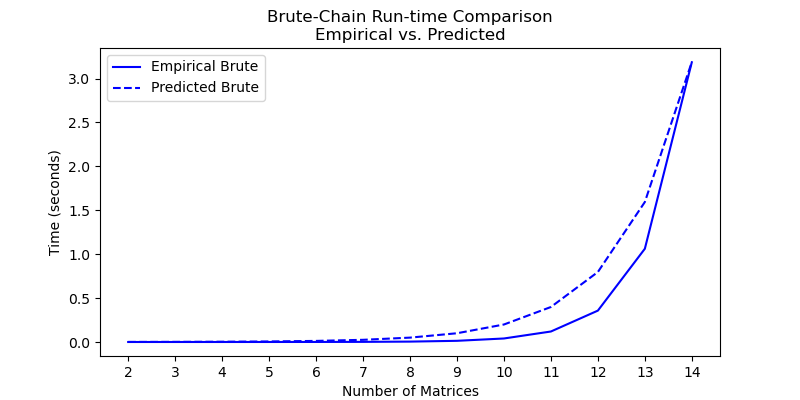
\includegraphics[scale=.8]{Analysis of Algs/brute_emp_vs_pred.png}
    \caption{Empirical run-time compared with predicted run-time for Brute-Chain}
    \label{fig:brute-chain}
\end{figure}

\begin{figure}
    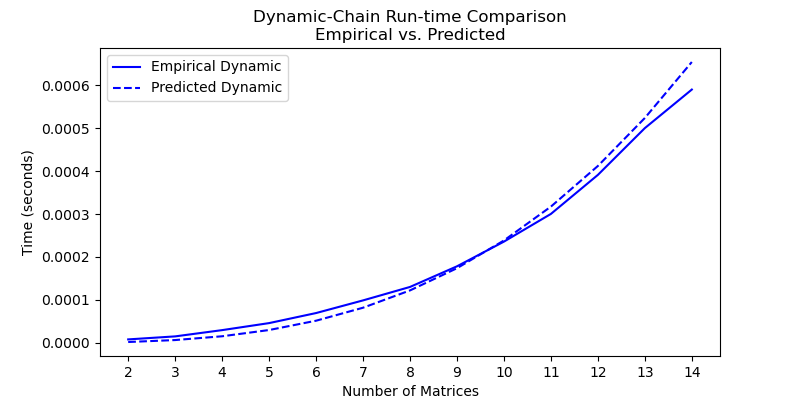
\includegraphics[scale=.8]{Analysis of Algs/dynamic_emp_vs_pred.png} 
    \caption{Empirical run-time compared with predicted run-time for Dynamic-Chain}
    \label{fig:dynamic-chain}
\end{figure}

\begin{figure}
    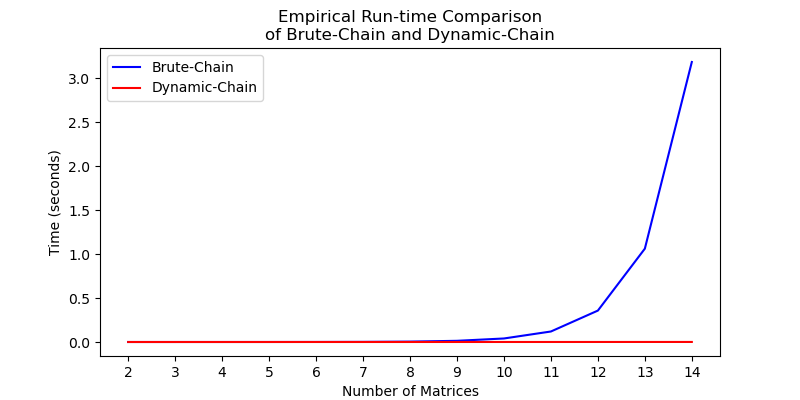
\includegraphics[scale=.8]{Analysis of Algs/brute_vs_dynamic.png}  
    \caption{Empirical run-time of Brute-Chain compared with Empirical run-time of Dynamic-Chain}
    \label{fig:brute_vs_dynamic}
\end{figure}



\section{Conclusion}
I have confirmed empirically that the dynamic programming approach to solving the matrix chain multiplication problem is far more efficient than a brute force approach. It is incredible to see that brute force becomes infeasible in real application when the number of matrices in the chain exceeds 16 because the run time doubles for every matrix multiplied into the chain. Dynamic programming keeps the run-time at a reasonable $O(n^3)$. Thus, it is a fruitful technique to use in problems that require optimizing subproblems and when subproblems overlap often. The matrix chain multiplication problem is a clear example of the utility of dynamic programming.

\begin{thebibliography}{1}
  \bibitem{CLRS} T. H. Cormen, C. E. Leiserson, R. L. Rivest, and C. Stein, {\em Introduction to Algorithms, 3rd edition}, The MIT Press, 2009, ISBN: 026203384.
  \bibitem{Chen} B. Chen, {\em Vector Spaces and Linear Transformations}, Fall 2006, https://www.math.ust.hk/~mabfchen/Math111/Week7-9.pdf
  
  \bibitem{muhammad} R. Muhammad, { \em Matrix-chain Multiplication Problem,} March 18, 2010, http://personal.kent.edu/~rmuhamma/Algorithms/MyAlgorithms/Dynamic/chainMatrixMult.htm
\end{thebibliography}
  
\end{document}